%%%%%%%%%%%%%%%%%%%%%%%%%%%%%%%%%%%%%%%%%%%%%%%%%%%%%%%%%%%%%%%%%%%%
%% chapter2.tex
%% UNL thesis document file
%%
%% Chapter with the template manual
%%%%%%%%%%%%%%%%%%%%%%%%%%%%%%%%%%%%%%%%%%%%%%%%%%%%%%%%%%%%%%%%%%%%
\chapter{Fundamentals}
\label{cha:fundamentals}

In this chapter the difference between verbal and non-verbal communication will be clarified. To understand what factors influence the quality of speech, in \ref{sec:anatomy} the anatomy of speech production will be explained.  



% ==================================================================
\section{Verbal vs. Non-verbal Communication} % (fold)
\label{sec:communication}


% ==================================================================
\section{Facial Muscles} % (fold)
\label{sec:anatomy}


The human face is composed by 43 muscles. Without them we would be missing an important tool for communicating not only with people from our cultural environment but also with people from different provenience as the only way to be understood would be through gestures. Our facial muscles are essential for both, verbal and non-verbal communication.\par 

\subsection{Speech Production Anatomy}
For verbal communication besides tongue, larynx, pharynx, and soft palate muscles, which are not visible from the exterior, also lip and mandibular muscles are crucial (orbicularis oris: close lips, levator labii superioris: raise upper lip, more in \cite{PhonManual}). 
Malfunction of these muscles can be caused by neurological or motoric problems, causing f.ex. speech disorders or facial paralysis. 

\subsection{Muscles of Facial Expression}

\begin{figure}
    \centering
    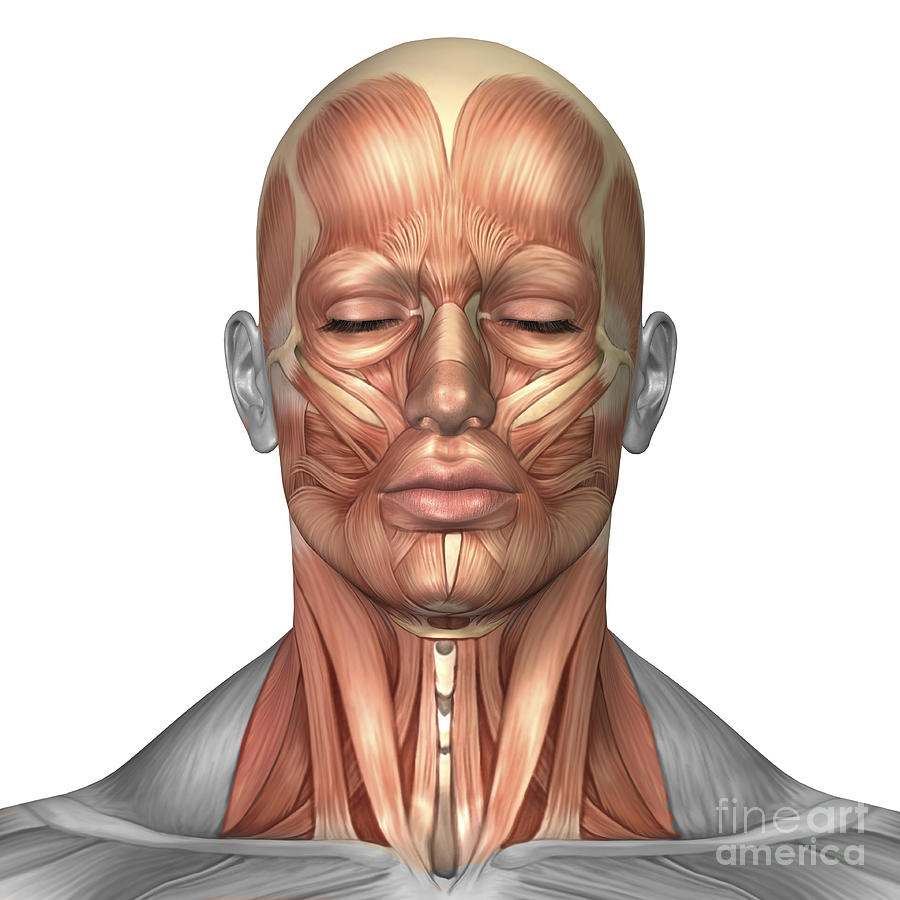
\includegraphics{faceAnatomy}
    \caption{Muscle anatomy of the human face (anterior view).\cite{FaceMuscles}}
    \label{fig:my_label}
\end{figure}

% ==================================================================
\section{Automatic Facial Expression Recognition}

\begin{figure}
{\footnotesize
\begin{forest}
    for tree={
      edge path={
        \noexpand\path [draw, thick, \forestoption{edge}] (!u.parent anchor) -- +(5pt,0) |- (.child anchor)\forestoption{edge label};
      },
      parent anchor=east,
      child anchor=west,
      grow'=east,
      text centered,
      minimum width=1in,
      text width=2.4cm
      }
 [Automatic\\  Facial\\ Expression Recognition [Parametrization [Descriptive] [Judgement]] [Recognition [Face \\ localization [Detection] [Segmentation]] [Face \\ registration] [Feature \\ extraction [Predesigned [Appearance][Geometry][Appearance + Geometry]][Learned]] [Expression\\ Classification /Regression [Categorical] [Continuous]] [Multimodal \\fusion [Direct fusion][Early fusion][Late fusion] [Sequential]]]]
  \end{forest}
}
\caption{Taxonomy for AFER adapted from \cite{Corneanu2016survey}.}
\label{fig:AFER}
\end{figure}

Automatic Facial Expression Recognition (AFER) is an interdisciplinary domain in which researchers from behavioural science, neurology, psychology, and computer science investigate the recognition of facial expressions which can give us insights about the emotional state of a person.

\subsection{Parametrization of FEs}




\subsection{Recognition of FEs}

\subsubsection{Face Localization}

\subsubsection{Face Registration}

\subsubsection{Feature Extraction}

\subsubsection{FE Classification and Regression}

\subsubsection{Multimodal Fusion Techniques}

\subsection{3D representations}
\cite{Sandbach2012survey}
\subsection{Thermal}


% ==================================================================
\section{Speech Language Pathology}
\label{sec:SLP}
\cite{SLPathologies}: prevalence in the US on page 10

Diagnosis and treatment of:\\
- swallowing (dysphagia) \\
- speech-language disorders\\
- cognitive-communication disorders\\


Speech-Language Pathologists treat disorders of:\\
- speech sound production (e.g., articulation, apraxia, dysarthria)\\
- resonance (e.g., hypernasality, hyponasality)\\
- voice (e.g., phonation quality, pitch, respiration)\\
- fluency (e.g., stuttering)\\
- language (e.g., comprehension, expression, pragmatics, semantics, syntax)\\
- cognition(e.g., attention, memory, problem solving, executive functioning)\\
- feeding and swallowing (e.g., oral, pharyngeal, and esophageal stages) \\

Some etiologies:\\
- neonatal problems (e.g., prematurity, low birth weight, substance exposure)\\
- developmental disabilities (e.g., specific language impairment, autism spectrum
disorder, dyslexia, attention deficit/hyperactive disorder)\\
- oral anomalies (e.g., cleft lip/palate, dental malocclusion, macroglossia, oral-motor
dysfunction)\\
- neurological disease/dysfunction (e.g., traumatic brain injury, cerebral palsy, cerebral
vascular accident, dementia, Parkinson's disease, amyotrophic lateral sclerosis)\\



% ==================================================================
\begin{comment}
\section{Example glossary and acronyms}
%
% \todo[inline]{A a note in a line by itself.}
%
This is the first occurrence of an abbreviation: \gls{abbrev}.

And now the second occurrence of the same abbreviation: \gls{abbrev}.

And a new acronym with capital letter: \Gls{xpt} and reused \gls{xpt}.

Lets add the term ``\gls{computer}'' to the glossary!

\end{comment}